Soit un langage régulier $L$. L'algorithme d'Angluin\cite{Angluin87} est un algorithme d'apprentissage actif d'automate qui permet d'apprendre un automate $A$ représentant $L(A)=L$. Il prend la forme d'un couple professeur/élève où :
\begin{itemize}
	\item L'élève applique l'algorithme d'Angluin $L^*$ en temps que tel pour construire un automate représentant le langage cible. Pour cela, il s'aide d'une table d'observation (section \ref{angluin:to})
	\item Le professeur a accès au langage que l'élève veut apprendre.
\end{itemize}

De plus, ce professeur contient deux oracles :
\begin{itemize}
	\item L'oracle d'appartenance. Soit un mot $w$. Appartient-il à $L$ ?
	\item L'oracle d'équivalence. Soit un automate $A_O$. Représente-t-il $L$ ? Si non, fournir un contre-exemple $w$.
\end{itemize}

\begin{figure}[H]
	\centering
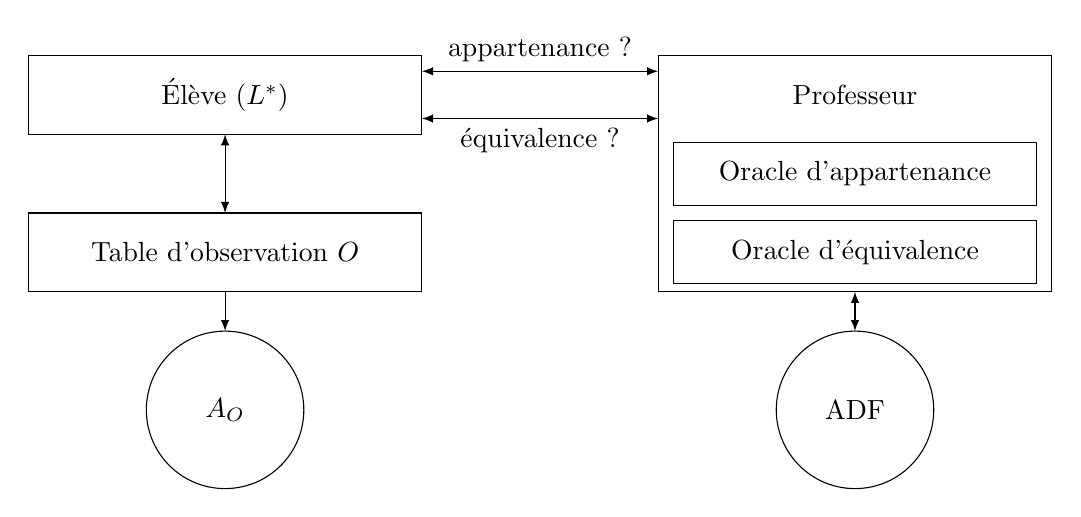
\begin{tikzpicture}
	\tikzset{>=latex}

	\draw (0,1) rectangle (5,0) node[pos=.5] {Élève ($L^*$)};
	\draw (8,1) rectangle (13,-2);

	\draw (8.2,-0.1) rectangle (12.8,-0.9) node[pos=.5] {Oracle d'appartenance};
	\draw (8.2,-1.1) rectangle (12.8,-1.9) node[pos=.5] {Oracle d'équivalence};

	\draw (0,-1) rectangle (5, -2) node[pos=.5] {Table d'observation $O$};

	\draw (10.5, -3.5) circle (1);
	\draw (2.5, -3.5) circle (1);

	\node[draw=none] at (10.5, 0.5) {Professeur} ;
	\node[draw=none] at (10.5,-3.5) {ADF};
	\node[draw=none] at (2.5,-3.5) {$A_O$};

	\draw[<->] (5,0.8) -- (8,0.8) node[pos=0.5,above] {appartenance ?};
	\draw[<->] (5,0.2) -- (8,0.2) node[pos=0.5,below] {équivalence ?};

	\draw[->] (2.5,-2) -- (2.5,-2.5);
	\draw[<->] (10.5, -2) -- (10.5,-2.5);
	\draw[<->] (2.5, 0) -- (2.5,-1);

\end{tikzpicture}
\caption{Vue schématique de l'algorithme d'Angluin}
\end{figure}

\begin{theorem}
	S'appuyant sur un professeur pour un langage régulier $L\subseteq\Sigma^*$, un élève peut utiliser l'algorithme d'Angluin $L^*$ pour apprendre l'ADF canonique $A$ représentant $L$ en un temps polynimial à $n$ le nombre d'états de $A$ et $m$ le nombre de contre-exemples reçus du professeur.
	Il effectue $\mathcal{O}(n)$ requêtes d'équivalence et $\mathcal{O}(mn^2)$ requêtes d'appartenance.\cite{Angluin87}
\end{theorem}

\begin{corollary}
	Si les requêtes d'appartenance et d'équivalence se font en temps polynomial en la taille de $A$, $L^*$ est en temps polynomial.
\end{corollary}

Attention cependant : cet algorithme part du postulat que le langage étudié est régulier.

Les prochaines section introduisent les différentes notions notemment necéssaires à la compréhension du fonctionnement de la table d'observation.
